\documentclass{article}

\usepackage[final, nonatbib]{neurips_2024}
\usepackage[numbers,compress]{natbib}
\usepackage[T1]{fontenc}
\usepackage[utf8]{inputenc}
\usepackage{amsmath,amssymb}
\usepackage{graphicx}
\usepackage{booktabs}
\usepackage{microtype}
\usepackage{hyperref}
\hypersetup{hidelinks}

\title{How Label-Efficient is the MNIST Record Holder?\\
       A Low-Data Benchmark and a Stacking Pitfall}

\author{%
  Attila Torda \\
  Independent Researcher
}

\begin{document}
\maketitle

\begin{abstract}
The reproducible MNIST CNN record holder---a majority vote of three ``simple'' CNNs---is
celebrated for accuracy ($99.87\%$), but its \emph{label efficiency} is rarely measured. On a
class-balanced low-label sweep ($n=20$ to $5000$, $5$ seeds) we find it is already near the
data-efficiency frontier: it reaches $64\%$ from $20$ labels and $90\%$ from $100$, and
\textbf{wins at every budget} against a strong, diverse ensemble of an interpretable
skeleton-graph classifier, a diffusion-augmented CNN, and the record holder's own networks. The
ensemble converges to within $\sim$2~pp by $n\!\geq\!1000$ but never overtakes. We then test
whether \emph{augmenting} the record holder with this structural and generative diversity helps,
and surface a methodological pitfall: a leakage-free stacker that reserves a held-out split to
fit its meta-learner \emph{starves the base learners of scarce labels}, inflating the apparent
ensemble gain by $\sim$3~pp at $n\!=\!100$--$200$. Measured against a baseline that keeps all its
labels, the gain shrinks to $+0.7$~pp or reverses. We release a reproducible benchmark and a
faithful light re-implementation of the record holder, and argue that low-data ensembling
results must be reported against full-budget baselines.
\end{abstract}

\section{Introduction}
Strong CNNs are near-perfect on MNIST \cite{LeCun1998}; the reproducible record is a majority
vote of three deep ``simple'' CNNs with kernels $3,5,7$, reaching $99.87\%$ \cite{An2020}. Two
questions are less studied. First, \emph{how label-efficient} is such a model---how far does it
fall at $20$, $100$, or $1000$ labels, and can a diverse ensemble of cheaper, decorrelated
learners beat it there? Second, if a single strong model cannot be beaten head-to-head, can it
be \emph{augmented} by adding structural and generative members? We benchmark both questions on a
class-balanced low-label sweep, contribute a faithful light re-implementation of the record
holder, and report an honest negative with a useful methodological lesson about low-data
stacking.

\section{Setup}
\paragraph{Models.} The \textbf{record holder} \cite{An2020} is re-implemented faithfully but
lightly (one model per kernel, fewer epochs); our repro reaches $99.65\%$ at $60$k (vs published
$99.87\%$). The \textbf{grand ensemble} stacks three decorrelated members: a skeleton-fusion CNN,
a $93$-dim skeleton-graph bag-of-features with a random forest \cite{Breiman2001,GuoHall1989},
and a CNN trained on images from a small class-conditional diffusion model
\cite{Ho2020,Song2021}; members are combined by leakage-free stacked generalisation
\cite{Wolpert1992}.
\paragraph{Protocol.} For each budget $n\in\{20,\dots,5000\}$ we sample exactly $n/10$ labels per
digit, train on the same budget, and evaluate on the full $10$k test set, averaged over $5$
seeds. The diffusion member is active only for $n\!\geq\!500$ (a DDPM cannot be trained on fewer
images).

\section{Results}
\paragraph{The record holder is the data-efficiency winner.}
Table~\ref{tab:eff} and Figure~\ref{fig:eff} show MNIST test accuracy across budgets. The record
holder wins at \emph{every} budget---most decisively in the extreme low-data regime ($64\%$ vs
$47\%$ at $n\!=\!20$), exactly where explicit structural priors were expected to help most. The
grand ensemble (with morphological augmentation) closes the gap monotonically, reaching within
$\sim$2~pp by $n\!\geq\!1000$, but never overtakes. Simple rotation/translation augmentation on a
deep CNN is more label-efficient than hand-crafted skeleton/structural features.

\begin{table}[t]
\caption{MNIST test accuracy (\%, mean over $5$ seeds). The record holder wins at every budget.}
\label{tab:eff}
\centering
\begin{tabular}{@{}lrrr@{}}
\toprule
$n$ & record holder & grand ensemble & grand ensemble + aug \\
\midrule
20    & \textbf{64.2} & 44.1 & 46.7 \\
50    & \textbf{83.4} & 58.4 & 61.3 \\
100   & \textbf{90.2} & 80.9 & 81.1 \\
200   & \textbf{96.2} & 86.6 & 89.6 \\
500   & \textbf{98.2} & 92.6 & 95.5 \\
1000  & \textbf{98.8} & 95.0 & 96.9 \\
2000  & \textbf{99.1} & 96.7 & 98.0 \\
5000  & \textbf{99.4} & 97.8 & 98.7 \\
60000 & \textbf{99.65}& --- & --- \\
\bottomrule
\end{tabular}
\end{table}

\paragraph{Augmenting the record holder, and a stacking pitfall.}
If the ensemble cannot win head-to-head, can its members \emph{augment} the record holder? We
stack the record holder's M3/M5/M7 with the structural and diffusion members
(Figure~\ref{fig:aug}). A leakage-free stacker fits its meta-learner on a held-out $30\%$ of the
budget, so the base learners see only $70\%$. Against \emph{that} (weakened) record-holder
baseline the augmented model appears to gain $+4.2$~pp at $n\!=\!100$ and $+2.1$ at $n\!=\!200$.
But the comparison is unfair: the baseline was starved of labels. Measured against a record
holder that keeps \emph{all} $n$ labels (Table~\ref{tab:pitfall}), the gain shrinks to $+0.7$~pp
at $n\!=\!100$ and \emph{reverses} to $-0.9$ at $n\!=\!200$. Most of the apparent ensemble gain
was the held-out split silently recovering, not new signal.

\begin{table}[t]
\caption{The held-out-split pitfall. ``Apparent'' compares the augmented model to a stacker
baseline trained on $70\%$ of labels; ``true'' compares it to a record holder trained on all
$n$ labels. The apparent low-data gain is largely an artefact.}
\label{tab:pitfall}
\centering
\begin{tabular}{@{}lrrrrr@{}}
\toprule
$n$ & augmented & baseline ($70\%$) & apparent $\Delta$ & record holder (full $n$) & true $\Delta$ \\
\midrule
100 & 90.9 & 86.7 & $+4.2$ & 90.2 & $+0.7$ \\
200 & 95.4 & 93.2 & $+2.1$ & 96.2 & $-0.9$ \\
500 & 97.6 & 97.6 & $+0.1$ & 98.2 & $-0.6$ \\
\bottomrule
\end{tabular}
\end{table}

\begin{figure}[t]
\centering
\begin{minipage}{0.49\linewidth}\centering
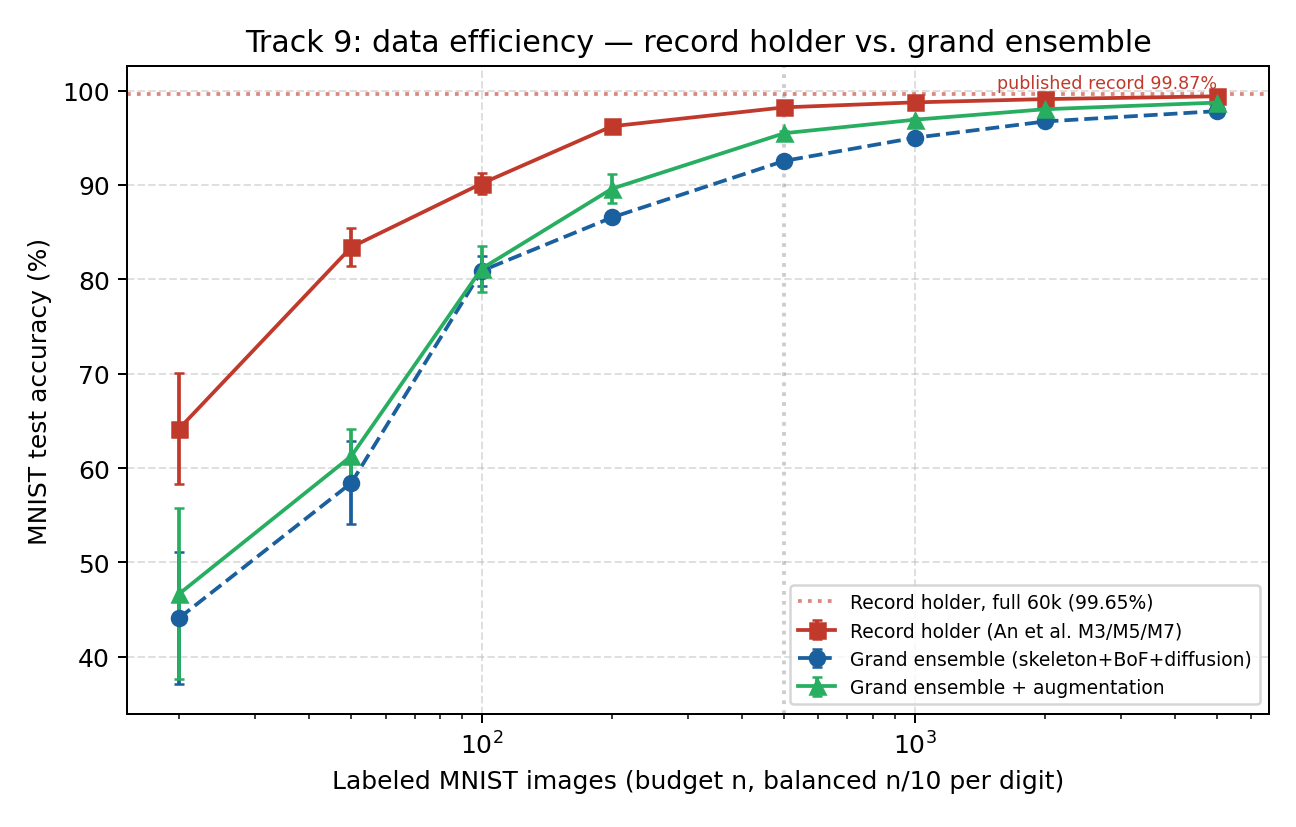
\includegraphics[width=\linewidth]{figures/fig7_track9_efficiency.png}
\end{minipage}\hfill
\begin{minipage}{0.49\linewidth}\centering
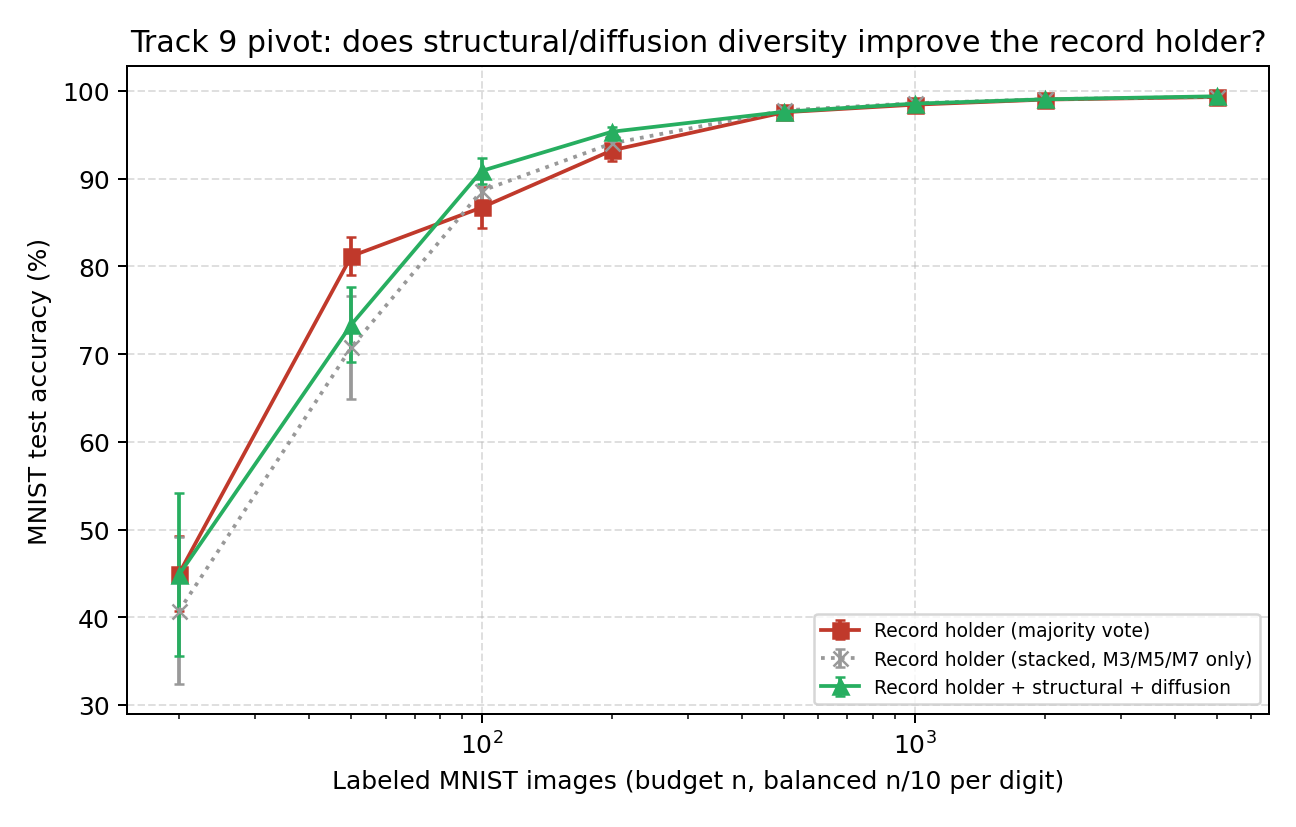
\includegraphics[width=\linewidth]{figures/fig8_track9_augment.png}
\end{minipage}
\caption{Left (\ref{fig:eff}): data-efficiency---the record holder (red) leads the grand ensemble
at every budget. Right (\ref{fig:aug}): augmenting the record holder; the apparent low-data gain
over the $70\%$-trained stacker baseline largely vanishes against a full-budget baseline.}
\label{fig:eff}
\label{fig:aug}
\end{figure}

\section{Discussion}
Two lessons. (1)~\textbf{SOTA CNNs are already near the label-efficiency frontier on MNIST}:
a diverse ensemble of structural and generative learners---each individually reasonable---does
not beat a well-tuned deep CNN ensemble at any budget down to $n\!=\!20$. Hand-crafted topology
helps less than geometric augmentation even when labels are scarcest. (2)~\textbf{Low-data
ensembling results must use full-budget baselines}: leakage-free stacking that reserves a held-out
split for the meta-learner systematically disadvantages the baseline by removing scarce labels,
and can manufacture a multi-point ``gain'' that is really label recovery. Held-out-free combiners
(soft or confidence-weighted averaging) avoid this and let every learner use all $n$ labels.

\textbf{Limitations.} A single dataset (MNIST) and a light record-holder repro ($99.65\%$ vs
$99.87\%$); $5$ seeds; the diffusion member needs $n\!\geq\!500$. The negative result is specific
to clean MNIST---under \emph{corruption}, corruption-agnostic structural/generative diversity
does help the record holder, which we study separately.

\section{Conclusion}
The MNIST record holder is remarkably label-efficient and is not beaten, nor cleanly augmented,
by structural and generative diversity in the clean low-data regime. The apparent augmentation
gain is largely a held-out-split artefact. We release the benchmark and the record-holder repro,
and recommend full-budget baselines for all low-data ensembling claims.

\begin{ack}
Reproducibility: \texttt{scripts/run\_track9\_benchmark.py} (data efficiency),
\texttt{scripts/run\_track9\_augment.py} (augmentation + pitfall). Models: \texttt{src/track9/}.
Raw results: \texttt{track9\_results.json}, \texttt{track9\_augment\_results.json}.
\end{ack}

\bibliographystyle{plainnat}
\bibliography{track9_benchmark_refs}

\end{document}
